\documentclass[9pt, aspectratio=169]{beamer}
\usepackage{FiraSans}
\usetheme[subsectionpage=progressbar]{metropolis}
\usepackage[utf8]{inputenc}
\usepackage{amsmath}
\usepackage{amsfonts}
\usepackage{amssymb}
\usepackage{multicol}
\usepackage{tikz}
\usepackage{caption}
\usepackage{xcolor}
\usepackage[T1]{fontenc} 
\usepackage[skins]{tcolorbox}
\author{Nicola Roman\`o - nicola.romano@ed.ac.uk}
\title{Lecture 16 - Improving CNN performance}
\setlength{\fboxsep}{0pt}
\setbeamertemplate {footline}{\begin{scriptsize}\hfill\insertframenumber ~of \inserttotalframenumber\kern1em\vskip5pt\end{scriptsize}}

% Remove "Figure" in front of captions
% See https://tex.stackexchange.com/questions/82456/how-to-remove-figure-caption-prefix-figure-in-beamer
\captionsetup{labelformat=empty,labelsep=none}

\titlegraphic{\centering \includegraphics[scale=.5]{instituteLogo.png}}
\date{}

\begin{document}

\newtcolorbox{codebox}{enhanced,
    top=2pt,
    left=2pt,
    right=2pt,
    bottom=2pt,
    boxrule=0pt,
    leftrule=5pt,
    sharp corners,
    colback=gray!20,
    colframe=blue!60!black}

\begin{frame}
    \titlepage
\end{frame}

\begin{frame}
    {Learning objectives}
    \begin{columns}
        \begin{column}{0.8\textwidth}
            \begin{itemize}
                \item Describe common problems when training deep networks.
                \item Discuss good practices for generating good training data for deep networks.
                \item Describe and implement solutions to under/overfitting networks.
            \end{itemize}
        \end{column}
        \begin{column}{0.2\textwidth}
            
\includegraphics[angle=-30, origin=tr, width=1.5\textwidth]{lightbulb.png}
        \end{column}
    \end{columns}
\end{frame}

\section{Introduction}

\begin{frame}
    {Improving CNN performance}
    In the past lectures we have seen how to train a CNN to classify two \textit{standard datasets}, MNIST and CIFAR-10.

    These are good \textit{toy} examples, but they do not reflect nowadays real-world applications.

    In this and next lectures we will see how to improve the performance of CNN when using them on real-world datasets.
\end{frame}

\section{The problems}

\begin{frame}
    {Getting the right data}
    \begin{itemize}
        \item Providing good quality data is a key step in any ML project.
        \item Your CNN (or any other ML algorithm) will be trained on the data you provide, so any bias introduced there will be learned by the model.
        \item Obtaining a lot of good training data is expensive and not always possible.
    \end{itemize}

    \centering
    \textbf{How do we ensure data quality?}
\end{frame}

\begin{frame}
    {The bias-variance tradeoff}
    We want to train our model to perform some task. However, just like any statistical model, we don't want to \textbf{overfit}.

    \only<1-2>{\centering
        \includegraphics[width=.6\textwidth]{fitting.png}

        \raggedright
        In ML, we often describe this in terms of \textbf{bias} and \textbf{variance} errors.
        \pause
        \begin{itemize}
            \item \textbf{Bias} derives from erroneous assumptions in the learning algorithm. High bias can cause an algorithm to miss the relevant relations between features and target outputs (underfitting).
            \item \textbf{Variance} derives from sensitivity to small fluctuations in the training set. High variance may result from an algorithm modeling the random noise in the training data (overfitting).
        \end{itemize}
        \footnotesize(Adapted from Wikipedia)
    }
    \only<3->{
        \centering
        \includegraphics[width=.7\textwidth]{Bias_variance.jpg}

        \pause \textbf{How do we detect and fix under- and over-fitting?}
    }
\end{frame}

\begin{frame}
    {Selecting hyperparameters}
    \begin{itemize}
        \item Selecting the right hyperparameters is a crucial step in any ML project.
        \item The hyperparameters you choose will determine the performance of your model.
        \item There are a lot of hyperparameters to choose for a CNN, for example, number of hidden layers, number of nodes in each layer, number of filters, number of epochs, learning rate, etc.
    \end{itemize}

    \centering
    \textbf{How to find the best hyperparameters?} (next lecture)
\end{frame}

\section{Data quality}

\begin{frame}
    {Deep learning is an iterative process}

    Very often when you are building a deep learning model you will need to iterate through several version of your model to find the good one to use.

    \centering
    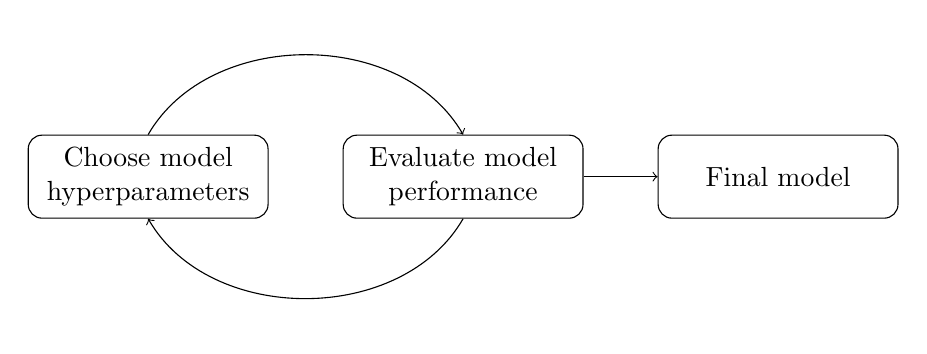
\begin{tikzpicture}
        \node[draw, fill=white, rectangle, rounded corners=5pt, text width=8em, align=center, minimum height=3em] (a) at (0,0) {Choose model hyperparameters};
        \node[draw, fill=white, rectangle, rounded corners=5pt, text width=8em, align=center, minimum height=3em] (b) at (4,0) {Evaluate model performance};
        \node[draw, fill=white, rectangle, rounded corners=5pt, text width=8em, align=center, minimum height=3em] (c) at (8,0) {Final model};

        \draw[->, in=120, out=60] (a.north) to (b.north);
        \draw[->, out=240, in=-60] (b.south) to (a.south);
        \draw[->] (b) to (c);
    \end{tikzpicture}
\end{frame}

\begin{frame}
    {Data splitting}
    We need to ensure our data is correctly split into training, validation and test sets.

    \centering
    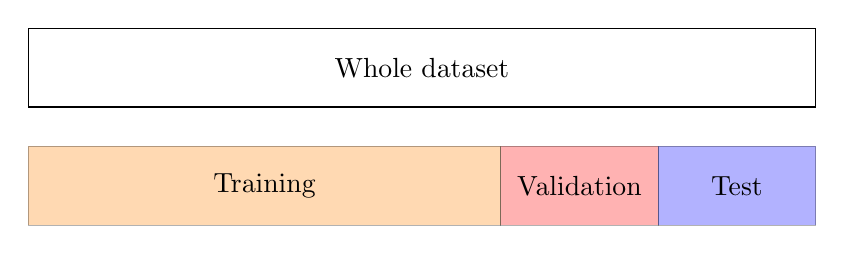
\begin{tikzpicture}
        \draw [fill=white] (0, 2.5) rectangle (10, 3.5);
        \node at (5, 3) {Whole dataset};
        \draw [fill=orange, opacity=0.3] (0, 1) rectangle (6, 2);
        \node[align=center] at (3, 1.5) {Training};
        \draw [fill=red, opacity=0.3] (6, 1) rectangle (8, 2);
        \node at (7, 1.5) {Validation};
        \draw [fill=blue, opacity=0.3] (8, 1) rectangle (10, 2);
        \node at (9, 1.5) {Test};
    \end{tikzpicture}

    \begin{itemize}
        \item Optimize the model by training it on the training set and evaluating it on the validation set.
        \item The validation set is not seen during training, so we can compare multiple models by evaluating them on it.
        \item Once we have a final model we can evaluate it on the test set.
              \pause
        \item In Python you can use the \texttt{test\_train\_split} function in \texttt{sklearn.model\_selection} module to split your data into training and test set (call it twice to further split the training set into training and validation).
    \end{itemize}
\end{frame}

\begin{frame}
    {How to split the data?}
    \begin{itemize}
        \item Traditionally, 60/20/20 (or 70/20/10) train/validation/test split has been used.
        \item If you are dealing with extremely large datasets (millions or hundreds of millions of observations) you will probably use much smaller validation and test sets.
        \item In those cases maybe 98\% or even more can be used as training set, since you will still have enough data in the validation and test set.
    \end{itemize}
\end{frame}

\begin{frame}
    {Match training and test set}
    It is important to train the model with data that is similar to the test data (and to the new data you want to use the model on).

    Sometimes training data is hard to come by and training is performed using available sources that might not match your own data.

    This might make your model inefficient.
\end{frame}

\begin{frame}
    {Data augmentation}
    What if you only have a small amount of training data?

    You can use \textbf{data augmentation} to increase the amount of training data you have, by generating synthetic data!

    For images, data augmentation is done by rotating, flipping, and cropping or otherwise distorting the images.
\end{frame}

\begin{frame}
    {Data augmentation - an example}
    \centering \includegraphics[width=\textwidth]{data augmentation.png}

    The original image (left) can be flipped, rotated,cropped etc.

    \pause
    \begin{columns}
        \begin{column}{.5\textwidth}
            \centering
            Make sure your augmentation makes sense!

            \includegraphics[width=.5\textwidth]{data augmentation wrong.png}
        \end{column}
        \pause

        \begin{column}{.5\textwidth}
            \centering
            This is fine, though!
            \includegraphics[width=\textwidth]{cellsupsidedown.png}
        \end{column}

    \end{columns}
\end{frame}

\begin{frame}
    {Augmentation in Keras}
    Keras 3 provides a new set of layers for data augmentation.
    These include the \texttt{RandomFlip}, \texttt{RandomRotation}, \texttt{RandomContrast} (and many more!) layers.

    See the documentation for more information on the \href{https://keras.io/api/layers/preprocessing_layers/image_augmentation/}{\underline{Image augmentation layers}}

    \pause
    These layers can be integrated into the model, so that the data is augmented on the fly during training!
\end{frame}

\begin{frame}
    {Dealing with unbalanced datasets}

    In classification problems a common problem is that the classes are not equally represented.

    For example, you might build a CNN to classify different types of cells. However, you might only have a small amount of cells for a specific type.
    
    If you randomly sample the data for your training set you might not have enough information to classify that cell type.

    Solutions to this problem are:

    \begin{itemize}
        \item Balance the dataset by sampling the data in a skewed way. Problem: you might not have enough data to train the model.
        \item Create augmented data only for the rare classes.
        \item Collect more data! 
    \end{itemize}
\end{frame}

\begin{frame}
    {Data preprocessing}
    In most cases you will want to scale your data.

    Networks using unscaled data can be very slow to train.

    The most used transformations used in deep learning are:

    \begin{itemize}
        \item \texttt{min-max normalization} - scale between 0 and 1
        \item \texttt{standardization} - scale to mean 0 and standard deviation 1
    \end{itemize}

    These can be performed, for example, using the \texttt{MinMaxScaler} and \texttt{StandardScaler} classes in the \texttt{sklearn.preprocessing} module.
\end{frame}

\section{Underfitting and overfitting}

\begin{frame}
    {Detecting underfitting/overfitting in a CNN}

    Plotting the loss during training can help you detect underfitting and overfitting.

    \centering
    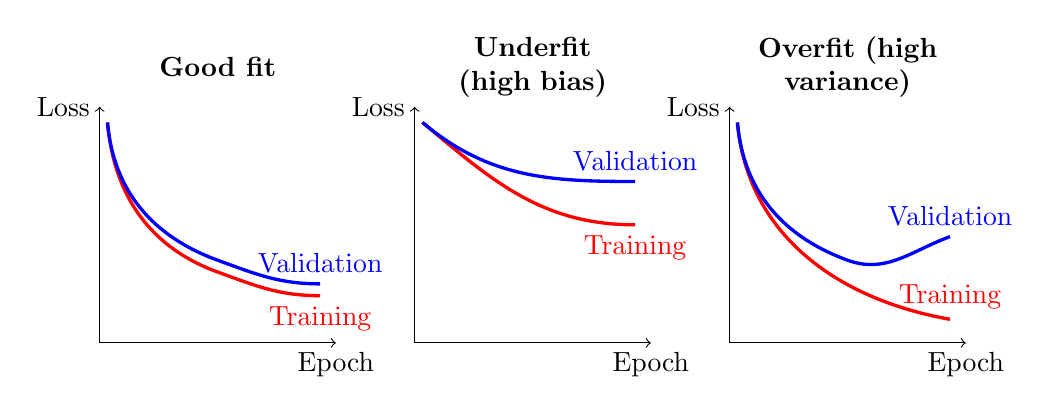
\begin{tikzpicture}
        % Axes
        \draw[<->] (0,3) node[left]{Loss} -- (0,0) -- (3,0) node[below]{Epoch};
        \draw[<->] (4,3) node[left]{Loss} -- (4,0) -- (7,0) node[below]{Epoch};
        \draw[<->] (8,3) node[left]{Loss} -- (8,0) -- (11,0) node[below]{Epoch};

        % Titles
        \node [align=center] at (1.5,3.5) {\textbf{Good fit}};
        \node [align=center, text width=8em] at (5.5,3.5) {\textbf{Underfit (high bias)}};
        \node [align=center, text width=8em] at (9.5,3.5) {\textbf{Overfit (high variance)}};

        % Good fit
        \draw [color=red, very thick] (0.1, 2.8) to [out=275, in=160] (1.5, 0.9) to [out=-20, in=180] (2.8, 0.6) node [below] {Training};
        \draw [color=blue, very thick] (0.1, 2.8) to [out=275, in=160] (1.5, 1.05) to [out=-20, in=180] (2.8, 0.75) node [above] {Validation};

        % Underfit
        \draw [color=red, very thick] (4.1, 2.8) to [out=-40, in=180] (6.8, 1.5) node [below] {Training};
        \draw [color=blue, very thick] (4.1, 2.8) to [out=-40, in=180] (6.8, 2.05) node [above] {Validation};

        % Overfit
        \draw [color=red, very thick] (8.1, 2.8) to [out=275, in=170] (10.8, 0.3) node [above] {Training};
        \draw [color=blue, very thick] (8.1, 2.8) to [out=275, in=160] (9.5, 1.05) to [out=-20, in=200] (10.8, 1.35) node [above] {Validation};

    \end{tikzpicture}

    \pause
    \textbf{How do we solve these problems?}
\end{frame}

\begin{frame}
    {Underfitting}
    Underfitting generally derives from the model being too simple and not being able to learn how to solve the problem.

    \begin{itemize}[<+->]
        \item The model is too shallow.\\\textit{Solution}: Increase the number of layers.
        \item Not enough features.\\\textit{Solution}: Increase the number of filters.
        \item Too short training.\\\textit{Solution}: train for more epochs.
        \item Learning rate too low.\\\textit{Solution}: Increase the learning rate.
    \end{itemize}
\end{frame}

\begin{frame}
    {Overfitting}
    Overfitting is often the result of a model that is too complex, learns from the training data too well, and is not able to generalise.

    \begin{itemize}
        \item Not enough training data.\\\textit{Solution}: Increase the size of the training set, gather more data, use image augmentation.
        \item Model is too complex.\\\textit{Solution}:Use dropout or regularization.
        \item Model trained for too long.\\\textit{Solution}: Use early stopping.
    \end{itemize}
\end{frame}

\begin{frame}
    {Weight regularization}
    To simplify the model, you can use weight regularization.
    This is a technique that pushes the weights of the model to be small.

    This is done by adding a \textit{cost} to the loss function that penalizes large weights (weighted by a constant $\lambda$).

    \Large
    $$J = \text{error}(y, \hat y) + \lambda ~ \text{cost}$$

    \normalsize
    Two types of regularization are commonly used:

    \begin{itemize}
        \item L1 regularization: the cost added to the loss is proportional to the sum of the absolute values of the weights (i.e. to the \textit{L1 norm} of the weight).
        \item L2 regularization: the cost added to the loss is proportional to the sum of the squares of the weights (i.e. to the \textit{L2 norm} of the weight).
    \end{itemize}
\end{frame}

\begin{frame}
    {Weight regularization in Keras}
    To add L1 or L2 regularization to a layer in Keras, you can set the \texttt{kernel\_regularizer} parameter when creating the layer.

    For example

    \begin{codebox}
        \texttt{layer = keras.layers.Dense(\\
            $~~~~$units=64,\\
            $~~~~$activation='relu',\\
            $~~~~$kernel\_regularizer=keras.regularizers.l1(0.01))
        }
    \end{codebox}
\end{frame}

\begin{frame}
    {Dropout}
    \begin{itemize}
        \item A type of "regularization" technique, used to prevent overfitting
        \item A random subset of the weights is set to zero at each training step.
        \item Originally introduced in "Dropout: A Simple Way to Prevent Neural Networks from Overfitting", Srivastava et al. 2014
    \end{itemize}

    \centering
    \only<1>{
        \includegraphics[width=\textwidth]{dropout.png}
    }
    \only<2>{
        \includegraphics[width=.5\textwidth]{dropout_error.png}
    }

    \footnotesize
    \raggedright
    Srivastava et al. 2014
\end{frame}

\begin{frame}
    {Early stopping}
    Early stopping is a technique that stops the training of a model if the validation loss does not improve for a certain number of epochs.

    It's easily implemented through the \texttt{EarlyStopping} Keras callback.

    \begin{codebox}
        \texttt{\# Create a callback that stops training when there is no improvement in the validation loss in 3 epochs\\
            early\_stop = tf.keras.callbacks.EarlyStopping(monitor='loss', patience=3)\\
            \# Train the model\\
            model.fit(x\_train, y\_train,\\
            $~~~~$epochs=100,\\
            $~~~~$validation\_data=(x\_val, y\_val),\\
            $~~~~$callbacks=[early\_stop])
        }
    \end{codebox}

\end{frame}

\end{document}

